% !TEX root = ./Basilisk-avsLibrary20170812.tex




\section{Library Description}
The AVS lab has released a set of astrodynamics C-functions\footnote{\url{http://hanspeterschaub.info/AVS-Code.html}} that facilitate common orbital or rotational dynamics evaluations.  The functions are openly available, and are included with the AIAA Education Series textbook \emph{Analytical Mechanics of Space Systems}\cite{schaub} since the first release in 2003.  The most up to date public versions are found on the AVS web page.

\subsection{{\tt linearAlgebra} Library}
The linear algebra library provides numerous C-based functions to perform basic matrix math operations.  For a complete list of functions supported, consult the {\tt linearAlgebra.h} file.   The library provides common matrix and vector manipulations tools such as performing a matrix product, including the transpose operators, as well as doing the matrix inverse operations.  The vector library supports doing dot and cross product operations, as well as taking a norms.  Helper functions are provided to initial zero or identity matrices, as well as check if the matrix elements are zero





\subsection{{\tt rigidBodyKinematics} Library}
The rigid body kinematics library provides a range of functions related to mapping between attitude coordinates descriptions, compute the addition or subtraction of orientations, as well as returning the differential kinematic equations.  This library has been included with Reference~\citenum{schaub} since 2003 and has been used extensively across a range of research projects.  Reference~\citenum{schaub} provides all the mathematical details of the transformation used here in Chapter 3, while Appendix E provides a comprehensive discussion of all the algorithms included.



\subsection{{\tt orbitalMotion} Library}
Common celestial mechanics tools are implemented in the {\tt orbitalMotion} library, including transforming between anomaly angles, converting between inertial Cartesian position and velocity vector components and classical orbit elements, as well as evaluating simple space environment parameters.  The following developments use the notation and formulation of Chapter 9 in Reference~\citenum{schaub}.  The variable naming is reflected within the software code.  


\subsubsection{Classical Orbital Elements}
The classcial orbit elements are given by 
$$
	(a, e, i, \Omega, \omega, f)
$$
where $a$ is the semi-major axis or SMA, $e$ is the eccentricity, $(\Omega, i, \omega)$ are the 3-1-3 Euler angle orbit plan orientation angles called the ascending node $\Omega$, the inclination angle $i$ and the argument of periapses $\omega$ which are illustrated in Figure~\ref{fig:orbit313}.   The semi-latus rectum $p$ is defined as
\begin{equation}
	p = a (1-e^{2})
\end{equation}
\begin{figure}[t]
	\centering
	\subfigure[Orbit Frame Orientation Illustration]
	{\label{fig:orbit313} 
	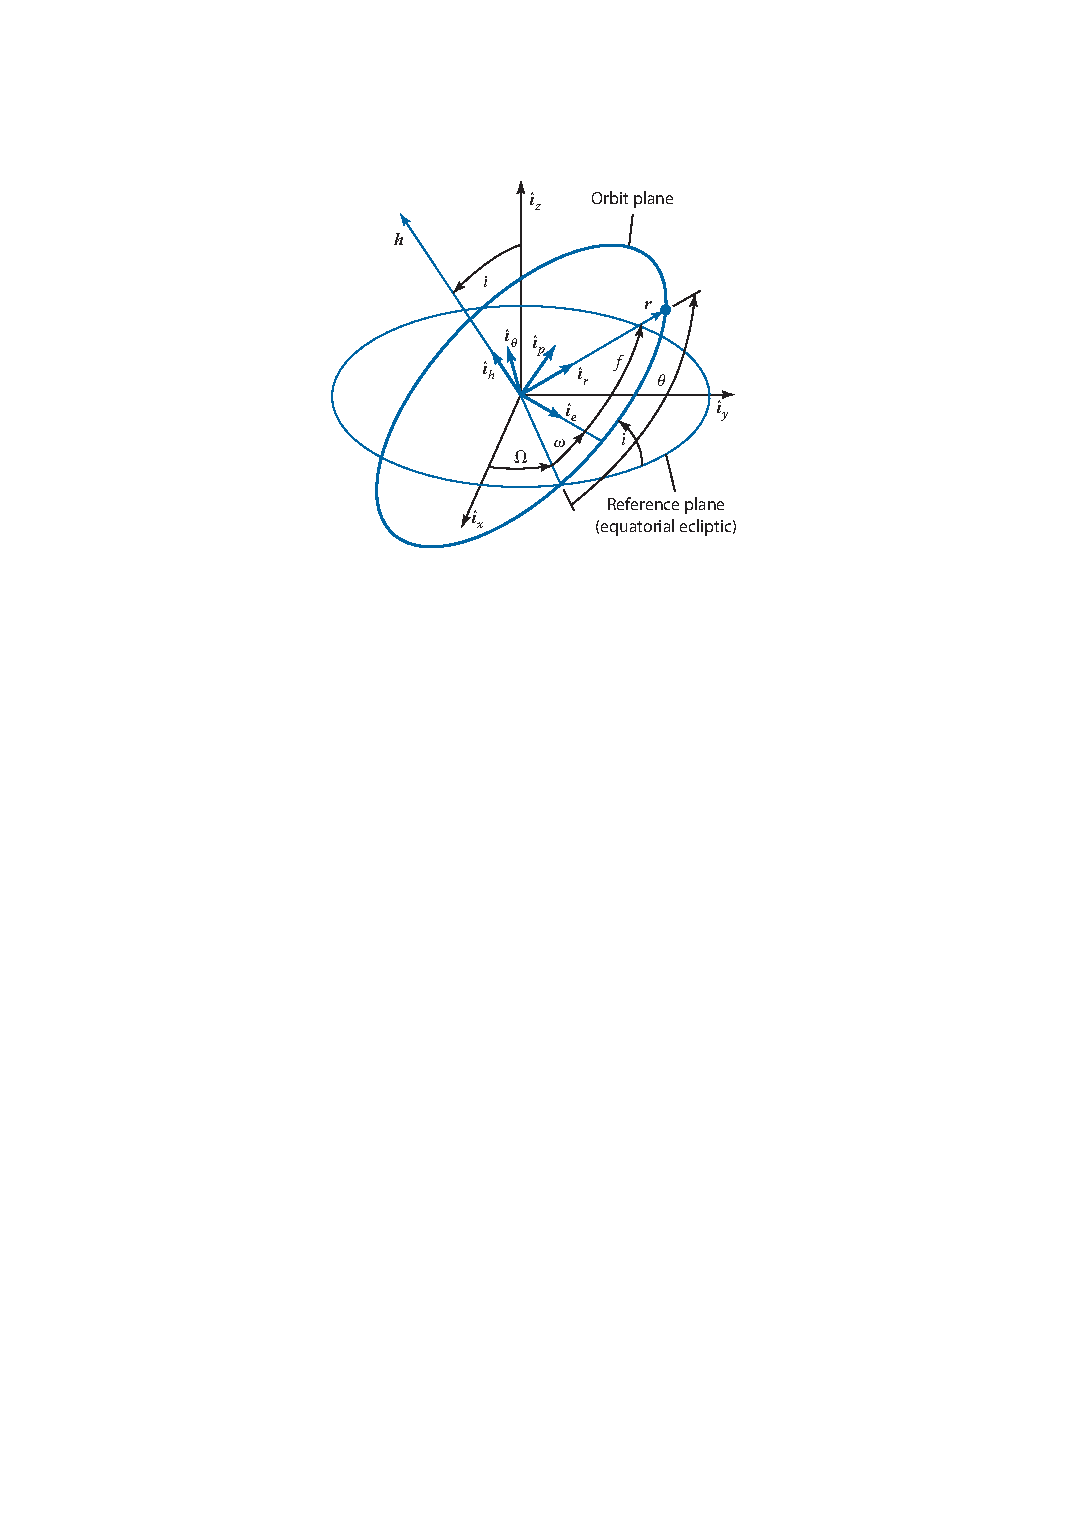
\includegraphics[width=0.45\textwidth]{Figures/orbit313}}  	
	\\	
	\subfigure[Classical orbital parameter Illustration for an Elliptic Orbit]
	{\label{fig:orbitElliptic}
	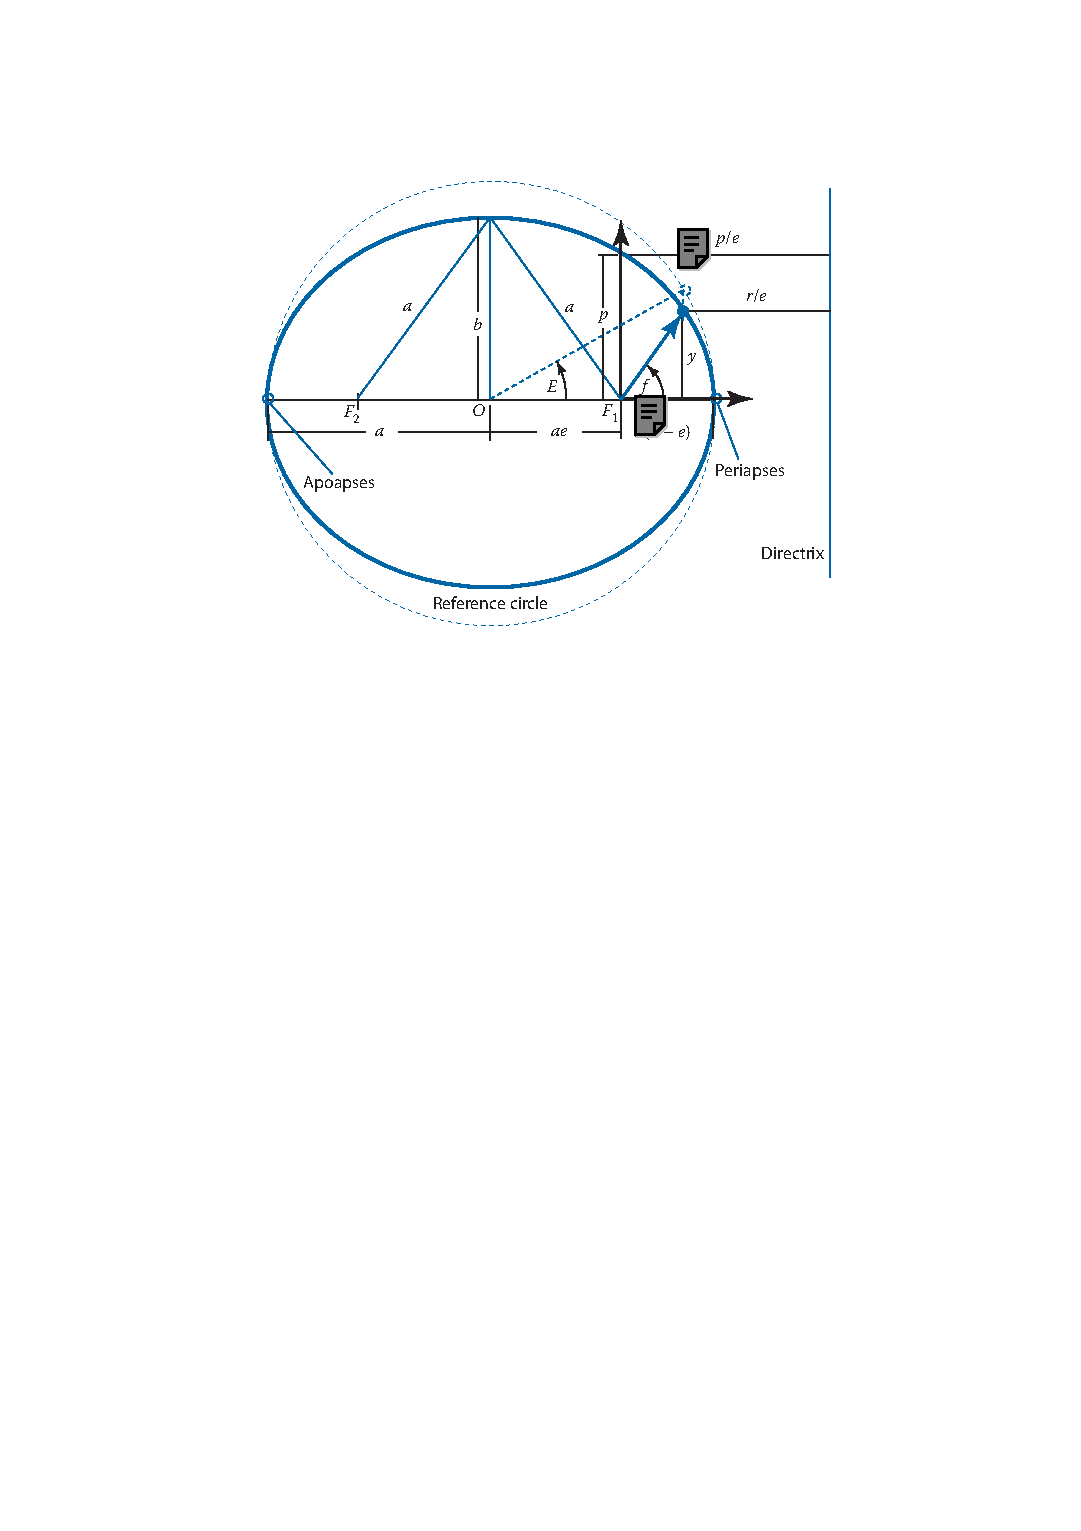
\includegraphics[width=0.45\textwidth]{Figures/orbitEllipse}} 
	\subfigure[Classical orbital parameter Illustration for a Hyperbolic Orbit]
	{\label{fig:orbitHyperbolic} 
	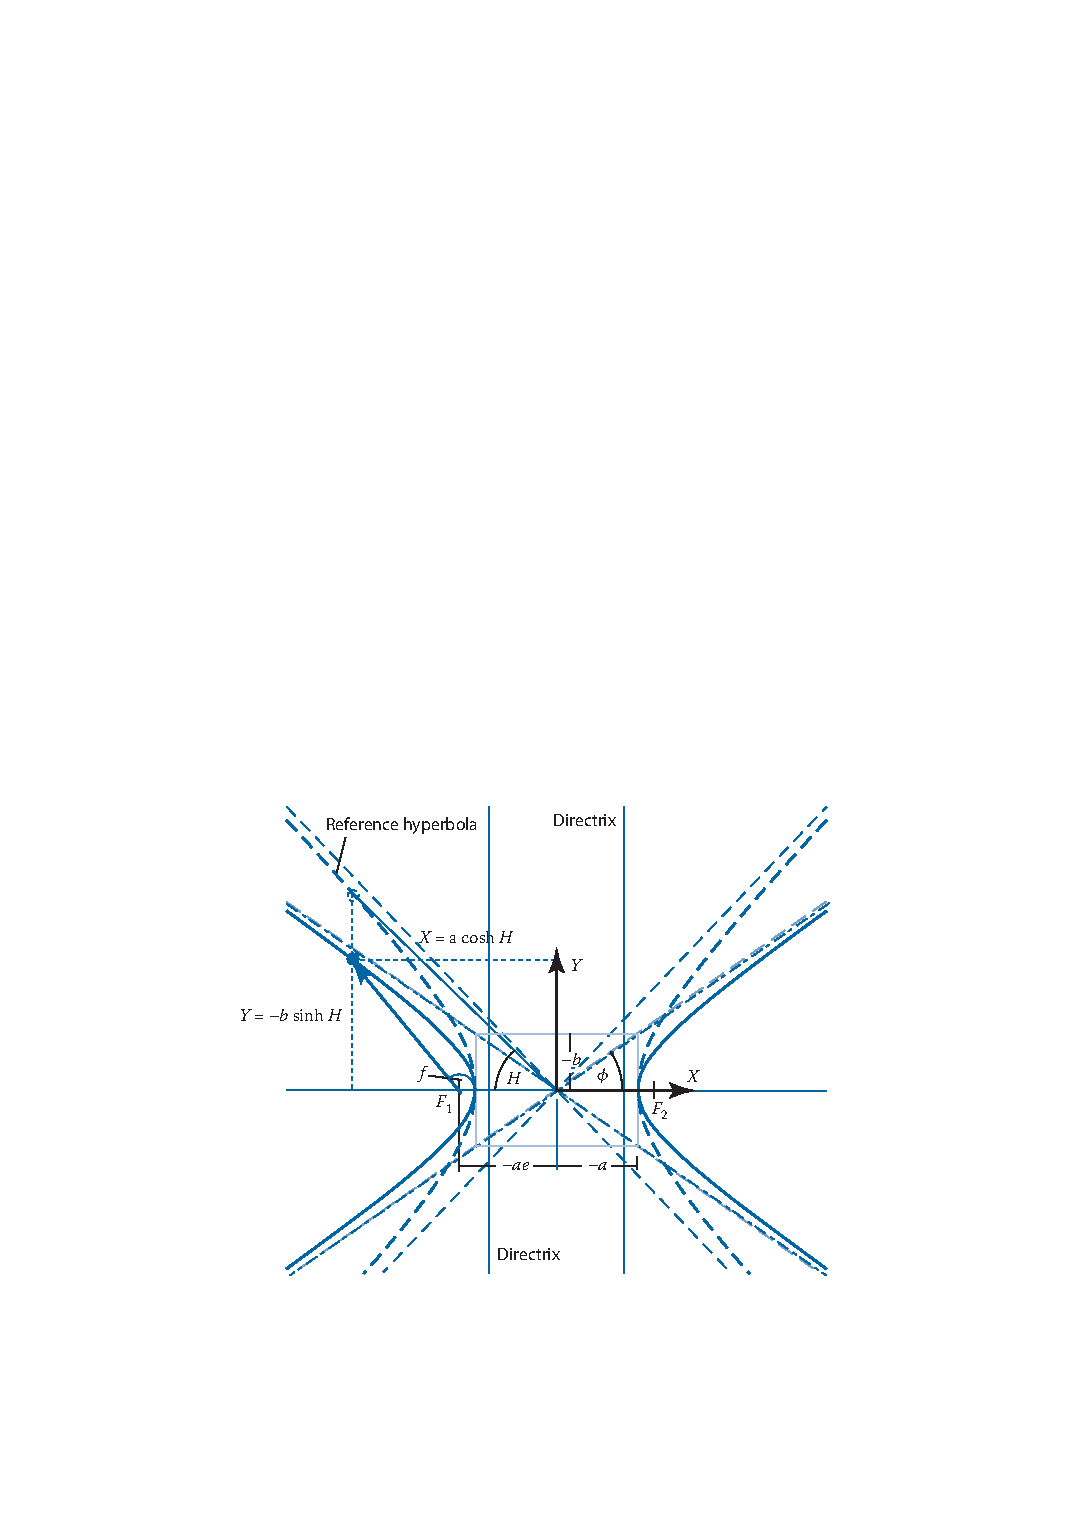
\includegraphics[width=0.45\textwidth]{Figures/orbitHyperbola}}  
	\caption{Orbit Elements, Axes and Frames Illustrations.\cite{schaub}}
	\label{fig:orbitParameters}
\end{figure}

Finally, the true anomaly angle is given by $f$, while the eccentric anomaly angle is expressed through $E$ as illustrated in Figure~\ref{fig:orbitElliptic} for an elliptic orbit scenario.  The true and eccentric anomaly are related through\cite{schaub}
\begin{equation}
	\tan\left( \frac{f}{2} \right) = \sqrt{ \frac{1+e}{1-e} } \tan\left( \frac{E}{2} \right) 
\end{equation}
The mean anomaly angle $M$ relates to the eccentric anomaly angle $E$ through\cite{schaub}
\begin{equation}
	M = E - e \sin E
\end{equation}

The classical orbit elements for a hyperbolic scenario are shown in Figure~\ref{fig:orbitHyperbolic}.  Note that the convention is used where the SMA is a negative value for a hyperbolic orbit, and thus $a < 0$ in this case.  The true anomaly angle $f$ definition is universal for all orbit types, while the hyperbolic anomaly $H$ relates to $f$ through
\begin{equation}
	\tanh\left( \frac{f}{2} \right) = \sqrt{ \frac{e+1}{e-1}} \tanh\left( \frac{h}{2} \right) 
\end{equation}
The hyperbolic mean anomaly is defined in terms of the hyperbolic anomaly through
\begin{equation}
	N = e \sinh H - H
\end{equation}


While mapping from to mean anomalies is analytical, the inverse is not.  The sub-routines use Newton's method to numerically solve from mean anomalies to the corresponding eccentric or hyperbolic anomalies.  This is called solving Kepler's equation.  The iterations continue until a change tolerance of $10^{-13}$ radians is achieved, or a maximum of 200 iterations are performed.  Note that solving this Kepler's equation for most cases converges very quickly within 3-5 iterations.  




\subsubsection{Orbit Element to Cartesian Coordinate Conversions}
Let $\leftexp{N}{\bm r}_{C/N}$ and $\leftexp{N}{\bm v}_{C/N}$ be the inertial spacecraft center of mass $C$ position and velocity vector matrix representations, expressed with respect to inertial frame \frameDefinition{N} components.  Functions are provided to map from classical orbit elements to these Cartesian coordinates through {\tt elem2rv()}, as well as the inverse mapping from Cartesian to classical orbit elements through {\tt rv2elem()}.  

\paragraph{{\tt elem2rv()} Function}
The general conversion of classical orbit elements to the inertial Cartesian components is outlined in detail in section 9.6.2 of Reference~\citenum{schaub}.  Given the true anomaly angle $f$, the orbit radius is for any orbit type given by
\begin{equation}
	r = \frac{p}{1 + e \cos f}
\end{equation}
The true latitude angle $\theta$ is given by
\begin{equation}
	\theta = \omega + f
\end{equation}
The inertial position vector is then given by\cite{schaub}
\begin{equation}
\bm r_{C/N} =r {\begin{matrix} ~ \\ ~ \\ ~
\end{matrix}}^{\cal N}\!\!\!\!  \begin{pmatrix}
\cos\Omega\cos\theta 
- \sin\Omega\sin\theta\cos i \\ 
\sin\Omega\cos\theta + \cos\Omega\sin\theta\cos 
i \\
 \sin\theta\sin i 
 \end{pmatrix}
\label{eq:tb:r2}
\end{equation}
while the inertial velocity vector is
\begin{equation}
\dot{\bm r}_{C/N} = -\frac{\mu}{h}
{\begin{matrix} ~ \\ ~ \\ ~
\end{matrix}}^{\cal N}\!\!\!\!  \begin{pmatrix}
\cos\Omega (\sin\theta + e\sin\omega ) + \sin\Omega 
(\cos\theta+e\cos\omega )\cos i \\
\sin\Omega (\sin\theta + e\sin\omega ) - \cos\Omega ( \cos\theta 
+ e\cos\omega )\cos i \\
-(\cos\theta + e\cos\omega )\sin i
\end{pmatrix}
\label{eq:tb:dr2}
\end{equation}
where $\mu$ is the gravitational constant and $h$ is the massless orbital angular momentum $\bm h = \bm r \times \dot{\bm r}$.  


The {\tt elem2rv()} function checks for a special rectilinear motion case.  Here the eccentricity is $e = 1$ while the SMA is positive with $a>0$.  Under this condition the spacecraft is moving purely along a radial direction relative to the planet, and the true anomaly angle no longer can be used to determine the spacecrafts location.  In this scenario the Eccentric anomaly angle $E$ can still be used to determine spacecraft position, and the {\tt elem2rv()} function assumes here that the anomaly angle provided is $E$ and not $f$.  The orbit radius is here computed using\cite{schaub}
\begin{equation}
	r = a (1 - e \cos E)
\end{equation}
The radial unit direction vector along which all rectilinear motion is occuring is
\begin{equation}
	\leftexp{N}{\hat{\bm\imath}}_{r}=\leftexp{N\!\!\!}{\begin{pmatrix}
\cos\Omega\cos\omega 
- \sin\Omega\sin\omega\cos i \\ 
\sin\Omega\cos\omega + \cos\Omega\sin\omega\cos 
i \\
 \sin\theta\sin i 
 \end{pmatrix}}
\end{equation}
The inertial position vector is then given by
\begin{equation}
\leftexp{N}{\bm r}_{C/N} =r \ \leftexp{N}{\hat{\bm\imath}}_{r}
\end{equation}


The velocity magnitude $v$ is determined through the orbit energy equation as\cite{schaub}
\begin{equation}
	v = \sqrt{ \frac{2 \mu}{r} - \frac{\mu}{a} }
\end{equation}
The inertial velocity vector is a function of the eccentric anomaly $E$ through
\begin{equation}
	\leftexp{N}{\bm v}_{C/N} = \begin{cases}
		-v \ \leftexp{N}{\hat{\bm\imath}}_{r}  & 0 \le E \le \pi \\
		+v  \ \leftexp{N}{\hat{\bm\imath}}_{r} & -\pi \le E \le 0
	\end{cases}
\end{equation}





\paragraph{{\tt rv2elem()} Function}
To convert from the inertial position and velocity vectors to the corresponding classical orbit elements, the following algorithm is used.  First the semi-latus rectum is computed using
\begin{equation}
	p = \frac{\bm h \cdot \bm h}{\mu}
\end{equation}
The line of nodes vector $\bm n$ is 
\begin{equation}
	\bm n = \hat{\bm n}_{3} \times \bm h
\end{equation}
The eccentricity vector $\bm e$ is computed using\cite{schaub}
\begin{equation}
	\bm e = \frac{\dot{\bm r} \times \bm h}{\mu} - \frac{\bm r}{r}
\end{equation}
The eccentricity is then simply
\begin{equation}
	e = |\bm e|
\end{equation}
Within this function the orbit radius is set through
\begin{equation}
	r = \frac{\bm r_{C/N}}{ | \bm r_{C/N}|}
\end{equation}
and the radius at periapses is set to
\begin{equation}
	r_{p} = \frac{p}{1 + e}
\end{equation}

The SMA is computed using a robust method where first the inverse of the SMA, called $\alpha$, is evaluated using\cite{schaub}
\begin{equation}
	\alpha = \frac{2}{r} - \frac{v^{2}}{\mu}
\end{equation}
If $\alpha$ is non-zero, then the orbit is not parabolic and $a$ is determined through
\begin{equation}
	a = \frac{1}{\alpha}
\end{equation}
while the radius at apoapses is set to
\begin{equation}
	r_{a} = \frac{p}{1 - e}
\end{equation}
If $\alpha$ is zero, then the motion is parabolic and the SMA is not defined (i.e. is infinite).  In this case the code sets 
$$
	a = -r_{p}
$$
while $r_{a} = -1.0$ is returned as a value that is not defined in this case.


Next the orbit frame orientation angles $\Omega$, $i$ and $\omega$ must be determined.  As classical elements are used, care must be given for particular singular orientations where some angles are ill-defined.  First, assume a non-circular non-equatorial orbit scenario.  In this case $\Omega$ is the angle between $\hat{\bm n}_{1}$ and $\bm n$ where care must be taken that the right quadrant is used.  The argument of periapses is the angle between $\hat{\bm n}$ and $\bm e$, where again quadrants must be checked.  Finally, the inclination angle $i$ is the angle between $\bm h$ and $\hat{\bm n}_{3}$, but here no quadrants must be checked as this angle is defined as $0 \le i \le \pi$.  To find the true anomaly angle, the angle between $\bm r$ and $\bm e$ is determine while checking for quadrants again.

The 3-1-3 Euler angles representing the orbit frame orientation have singular configurations.  The following list discusses how each case is handled:
\begin{itemize}
	\item {\bfseries Equatorial non-circular orbit:} Here the ascending node $\Omega$ is ill-defined, and is  set to 0.0 radians.  
	\item {\bfseries Inclined circular orbit:}  Here the argument of periapses $\omega$ is ill-defined, and is set to 0.0 radians.
	\item {\bfseries Equatorial circular orbit:} Here both $\Omega$ and $\omega$ are ill-defined are are each set to 0.0 radians.
\end{itemize}















\subsubsection{Space Environment Parameters}
\paragraph{Atmospheric Density}
This program computes the atmospheric density based on altitude  supplied by user.  This function uses a 7-th order polynomial curve fit based on  atmospheric data from the Standard Atmosphere 1976 Data. This function is valid for altitudes ranging from 100km to 1000km.

\paragraph{Mean Debye Length}
This program computes the Debye Length length for a given  altitude and is valid for altitudes ranging  from 200 km to GEO (35000km).  However, all values above   1000 km are HIGHLY speculative at this point.

\paragraph{Atmospheric Drag Acceleration}
This program computes the atmospheric drag acceleration   vector $\leftexp{N}{\bm a}_{d}$ acting on a spacecraft.   Note the acceleration vector output is inertial, and is   only valid for altitudes up to 1000 km.   Afterwards the drag force is zero. Only valid for Earth.  The disturbance acceleration is defined as
\begin{equation}
	\bm a_{d} = -\frac{\rho}{2} C_{d} \frac{A v^{2}}{m}
\end{equation}
where $\rho$ is the local atmospheric density, $C_{d}$ is the drag coefficient, $A$ is the projected area into the flight direction, and $m$ is the spacecraft mass.


\paragraph{Gravitational Zonal Harmonics}
This function computes Earth's zonal harmonics from $J_{2}$ through $J_{6}$.  For other planets only their $J_{2}$ value is used, while the higher order harmonics are set to zero.  The gravitational zonal harmonic accelerations are then given by\cite{schaub}
\begin{align}
	\bm a_{J_{2}} &=   -\frac{3}{2} J_{2} 
	\left(\frac{\mu}{r^{2}}\right)
	\left( \frac{r_{eq}}{r}\right)^{2}
	\begin{pmatrix}
		\left(1-5\left(\frac{z}{r}\right)^{2}\right) \frac{x}{r} \\
		\left(1-5\left(\frac{z}{r}\right)^{2}\right) \frac{y}{r} \\
		\left(3-5\left(\frac{z}{r}\right)^{2}\right) \frac{z}{r}
	\end{pmatrix}
	\label{eq:gm:aJ2}
	\\
	\bm a_{J_{3}} &=  -\frac{1}{2} J_{3} 
	\left(\frac{\mu}{r^{2}}\right)
	\left( \frac{r_{eq}}{r}\right)^{3}
	\begin{pmatrix}
		5\left(7 \left(\frac{z}{r}\right)^{3} - 3 \left(\frac{z}{r}\right) 
		\right) \frac{x}{r} \\
		5\left(7 \left(\frac{z}{r}\right)^{3} - 3 \left(\frac{z}{r}\right) 
		\right) \frac{y}{r} \\
		3\left(10\left(\frac{z}{r}\right)^{2} - \frac{35}{3} 
		\left(\frac{z}{r}\right)^{4} - 1 \right) 
	\end{pmatrix}
	\label{eq:gm:aJ3}
	\\
	\bm a_{J_{4}} &=  -\frac{5}{8} J_{4} 
	\left(\frac{\mu}{r^{2}}\right)
	\left( \frac{r_{eq}}{r}\right)^{4}
	\begin{pmatrix}
		\left(3-42 \left(\frac{z}{r}\right)^{2} +63 \left(\frac{z}{r}\right)^{4} 
		\right) \frac{x}{r} \\
		\left(3-42 \left(\frac{z}{r}\right)^{2} +63 \left(\frac{z}{r}\right)^{4} 
		\right) \frac{y}{r} \\
		-\left(15-70\left(\frac{z}{r}\right)^{2} + 63 
		\left(\frac{z}{r}\right)^{4}  \right) \frac{z}{r}
	\end{pmatrix}
	\label{eq:gm:aJ4}
	\\
	\bm a_{J_{5}} &=  -\frac{J_{5}}{8}  
	\left(\frac{\mu}{r^{2}}\right)
	\left( \frac{r_{eq}}{r}\right)^{5}
	\begin{pmatrix}
		3\left(35\left(\frac{z}{r}\right) - 210 
		\left(\frac{z}{r}\right)^{3} +231 \left(\frac{z}{r}\right)^{5}
		\right) \frac{x}{r} \\
		3\left(35\left(\frac{z}{r}\right) - 210 
		\left(\frac{z}{r}\right)^{3} +231 \left(\frac{z}{r}\right)^{5}
		\right) \frac{y}{r} \\
		\left(15- 315\left(\frac{z}{r}\right)^{2} \!\!+ 945 
		\left( \frac{z}{r}\right)^{4}\!\! -693 \left(\frac{z}{r}\right)^{6} 
		\right) 
	\end{pmatrix}
	\label{eq:gm:aJ5}
	\\
	\bm a_{J_{6}} &=  \frac{J_{6}}{16}  
	\left(\frac{\mu}{r^{2}}\right)\!
	\left( \frac{r_{eq}}{r}\right)^{6}\!
	\begin{pmatrix}
		\left(35 - 945 \left(\frac{z}{r}\right)^{2} \!\!
		+ 3465 \left(\frac{z}{r}\right)^{4} \!\!
		- 3003 \left(\frac{z}{r}\right)^{6} 
		\right) \frac{x}{r} \\
		\left(35 - 945 \left(\frac{z}{r}\right)^{2} \!\!
		+ 3465 \left(\frac{z}{r}\right)^{4} \!\!
		- 3003 \left(\frac{z}{r}\right)^{6}  
		\right) \frac{y}{r} \\
		\left( 3003 \left(\frac{z}{r}\right)^{6} \!\!
		-4851 \left(\frac{z}{r}\right)^{4}\!\!
		+ 2205 \left(\frac{z}{r}\right)^{2}\!\!
		- 315
		\right) \frac{z}{r}
	\end{pmatrix}
	\label{eq:gm:aJ6}
\end{align}

\paragraph{Solar Radiation Disturbance Acceleration}
A simple solar disturbance acceleration $\bm a_{d}$ function is implemented where
\begin{equation}
	\bm a_{d} = - \frac{C_{r} A \Pi}{m c s^{3}} \bm s
\end{equation}
where $C_{r} = 1.3$ is the radiation pressure coefficient,  $c = 299792458$m is the speed of light, $\Pi = 1372.5398$ W/m$^{2}$ is the solar radiation flux and $\bm s$ is the sun position vector relative to the spacecraft in units of AU.  



%120 linear algebra
%9 orbital anomalies
%8 orbital elements
%9 environment
%234 rigid body kinematics